% ============================================================
% KAPITEL 5 — IMPLEMENTIERUNG
% ============================================================

\chapter{Implementierung}
\label{ch:implementierung}

Dieses Kapitel beschreibt, wie das Konzept in ein lauffähiges System umgesetzt ist: den Aufbau im Überblick, die Anbindung der Szene, den Agenten mit seinen Werkzeugen, die fünf Repräsentationsvarianten und den VR-Demonstrator.


% ------------------------------------------------------------
\section{Systemüberblick}
\label{sec:impl-overview}

Das System verbindet einen natürlichsprachlichen Befehl mit einer sichtbaren Veränderung der 3D-Szene.
Es besteht aus drei lose gekoppelten Schichten, die über festgelegte Schnittstellen kommunizieren (Abbildung~\ref{fig:architektur}).

In der obersten Schicht deutet ein Agent den Befehl und wählt die nötige Manipulation.
Angetrieben wird er von einem lokal betriebenen Sprachmodell, für die visuelle Wahrnehmung greift er auf ein lokales visuelles Modell zurück.
Die mittlere Schicht ist ein Server nach dem Model Context Protocol (MCP)~\cite{mcp}.
Er stellt die Manipulationsoperationen als aufrufbare Werkzeuge bereit und übersetzt jeden Aufruf in eine Nachricht an die Umgebung; eine WebSocket-Verbindung transportiert diese Nachrichten und liefert Szenenzustand und gerenderte Bilder zurück.
Die unterste Schicht ist die Umgebung selbst, die die Szene hält, darstellt und die Manipulationen ausführt.
In der Evaluation läuft sie am Desktop, im Demonstrator auf der Meta Quest.
Weil die Schichten nur über diese Schnittstellen verbunden sind, lässt sich die Umgebung austauschen, ohne die übrigen Schichten zu verändern, und dieselbe Kette kann für die Messung und für den Demonstrator genutzt werden.

Ein Durchlauf beginnt mit dem Befehl an den Agenten.
Dieser fordert über die Werkzeuge zunächst den strukturellen Zustand oder eine gerenderte Ansicht an, entscheidet dann, welche Operation auszuführen ist, und ruft das passende Werkzeug auf.
Der MCP-Server leitet den Aufruf über die WebSocket-Verbindung an die Umgebung weiter, die die Manipulation ausführt.
Anschließend liest die Auswertung den neuen Szenenzustand aus und bestimmt daraus den Erfolg.

\begin{figure}[htbp]
  \centering
  \resizebox{\linewidth}{!}{%
  \begin{tikzpicture}[
      font=\small,
      box/.style={draw, rounded corners, align=center, inner sep=6pt,
                  minimum height=11mm, minimum width=27mm, fill=white},
      lbl/.style={font=\footnotesize, fill=white, inner sep=1.5pt},
      layer/.style={draw, dashed, rounded corners, inner sep=9pt},
      flow/.style={-{Latex[length=2.5mm]}, thick},
      back/.style={-{Latex[length=2.5mm]}, thick, dashed},
      exch/.style={{Latex[length=2mm]}-{Latex[length=2mm]}, thick},
      node distance=26mm and 30mm
    ]

    % --- Knoten ---
    \node[box] (user) {Nutzer\\{\footnotesize natürlichsprachlicher Befehl}};
    \node[box, below=of user] (agent) {Agent\\{\footnotesize (smolagents)}};
    \node[box, left=of agent]  (vlm) {Visuelles Modell\\{\footnotesize Qwen2.5-VL-7B}};
    \node[box, right=of agent] (llm) {Sprachmodell\\{\footnotesize Qwen2.5-7B}};
    \node[box, below=of agent] (mcp) {MCP-Server\\{\footnotesize (FastMCP)}};
    \node[box, below=of mcp]   (unity) {Unity-Umgebung\\{\footnotesize Szene, Rendering, Set-of-Mark}};

    % --- Nutzer -> Agent ---
    \draw[flow] (user) -- node[lbl, right]{Befehl} (agent);

    % --- Agent <-> Modelle ---
    \draw[exch] (agent) -- node[lbl, above]{Wahrnehmung} (vlm);
    \draw[exch] (agent) -- node[lbl, above]{Inferenz} (llm);

    % --- Agent <-> MCP ---
    \draw[flow] ([xshift=8mm]agent.south) -- node[lbl, right]{Werkzeugaufruf} ([xshift=8mm]mcp.north);
    \draw[back] ([xshift=-8mm]mcp.north)  -- node[lbl, left]{Ergebnis} ([xshift=-8mm]agent.south);

    % --- MCP <-> Unity ---
    \draw[flow] ([xshift=8mm]mcp.south)   -- node[lbl, right]{Kommando} ([xshift=8mm]unity.north);
    \draw[back] ([xshift=-8mm]unity.north)-- node[lbl, left, align=center]{Zustand /\\Bild} ([xshift=-8mm]mcp.south);

    % --- Schichten (Hintergrund) ---
    \begin{scope}[on background layer]
      \node[layer, fit=(vlm)(agent)(llm)] (L1) {};
      \node[layer, fit=(mcp)]   (L2) {};
      \node[layer, fit=(unity)] (L3) {};
    \end{scope}

    % --- Schicht-Beschriftungen ---
    \node[font=\footnotesize\itshape, anchor=east, xshift=-4mm] at (L1.west) {Agentenschicht};
    \node[font=\footnotesize\itshape, anchor=east, xshift=-4mm] at (L1.west |- L2) {Vermittlungsschicht};
    \node[font=\footnotesize\itshape, anchor=east, xshift=-4mm] at (L1.west |- L3) {Umgebungsschicht};

  \end{tikzpicture}%
  }
  \caption{Aufbau des Systems in drei Schichten und Nachrichtenfluss einer Manipulation. Durchgezogene Pfeile zeigen den Vorwärtsfluss, gestrichelte Pfeile den Rückkanal. Die Verbindung zwischen MCP-Server und Umgebung wird über WebSocket übertragen.}
  \label{fig:architektur}
\end{figure}


% ------------------------------------------------------------
\section{Szenenanbindung}
\label{sec:impl-scene}

Die Umgebung stellt die Szene in zwei Sichten bereit, einer strukturellen und einer visuellen.

Für die strukturelle Sicht führt die Umgebung intern ein Verzeichnis aller manipulierbaren Objekte und serialisiert es auf Anfrage als JSON.
Die Ausgabe enthält für jedes Objekt eine eindeutige Kennung, den Objekttyp, die Farbe, die Größe und die Position sowie zusätzlich die Pose der Kamera (Listing~\ref{lst:state}).
Die Kamerapose ist enthalten, damit sich auch Aufgaben lösen lassen, die sich auf den Betrachter beziehen.
Eigenschaften des Aussehens, die über die Grundfarbe hinausgehen, etwa eine Oberflächentextur, fehlen dagegen; deshalb sind rein perzeptuelle Referenzen über den strukturellen Zustand nicht auflösbar.

\begin{listing}[htbp]
\begin{minted}{json}
{
  "type": "state",
  "objects": [
    {"id": "obj_1", "type": "cube",   "color": "red",  "x": 0.0, "y": 0.0, "z": 0.0, "scale": 1.0},
    {"id": "obj_2", "type": "sphere", "color": "blue", "x": 2.0, "y": 0.0, "z": 0.0, "scale": 1.0}
  ],
  "camera": {
    "position": [0.0, 1.6, -6.0],
    "forward":  [0.0, 0.0, 1.0],
    "up":       [0.0, 1.0, 0.0]
  }
}
\end{minted}
\caption{Beispiel des strukturellen Szenenzustands als JSON-Ausgabe der Umgebung.}
\label{lst:state}
\end{listing}

Für die visuelle Sicht rendert die Umgebung die Szene aus der Kamera und übergibt das Bild.
Damit das visuelle Modell ein erkanntes Objekt auch für einen Werkzeugaufruf benennen kann, erhält jedes sichtbare Objekt nach dem Set-of-Mark-Prinzip~\cite{yang2023} eine gelbe, nummerierte Marke oberhalb seiner Bildposition.
Eine Zuordnungstabelle übersetzt die vom visuellen Modell genannten Nummern zurück in die Objektkennungen.
Beide Sichten verweisen damit auf dieselben Kennungen, sodass der Agent Objekte unabhängig von der Repräsentationsform einheitlich anspricht, wie es Abschnitt~\ref{sec:konz-fairness} verlangt.
Abbildung~\ref{fig:setofmark} zeigt dieselbe Szene ohne und mit Marken.

\begin{figure}[htbp]
  \centering
  \begin{minipage}{0.48\linewidth}
    \centering
    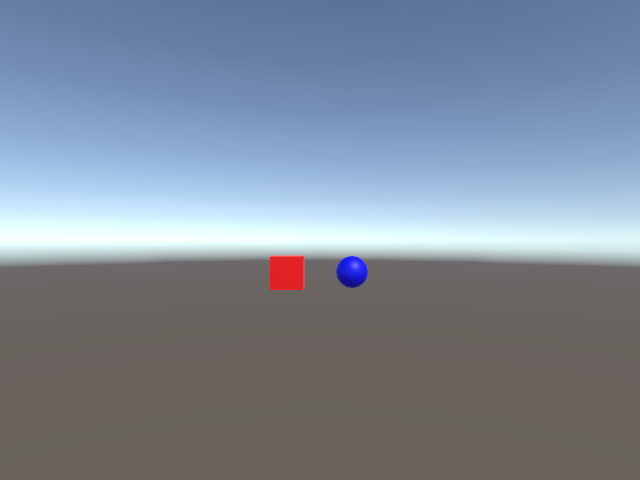
\includegraphics[width=\linewidth]{figures/scene}
  \end{minipage}\hfill
  \begin{minipage}{0.48\linewidth}
    \centering
    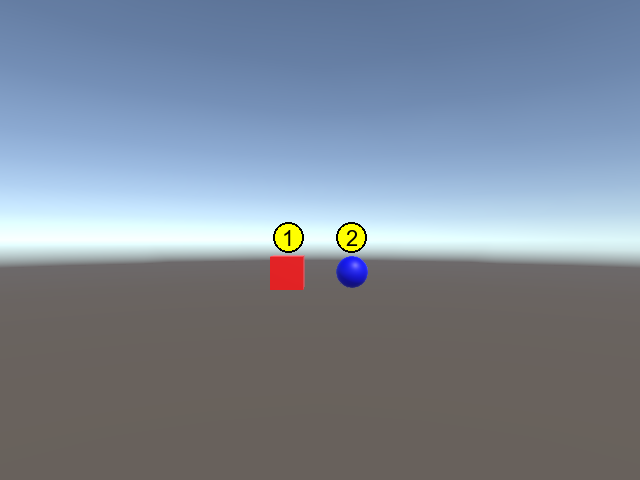
\includegraphics[width=\linewidth]{figures/scene_marked}
  \end{minipage}
  \caption{Die visuelle Repräsentation am Beispiel einer einfachen Szene. Links die gerenderte Ansicht, wie sie die Kamera liefert. Rechts dieselbe Ansicht nach dem Set-of-Mark-Verfahren, bei dem jedes sichtbare Objekt eine nummerierte Marke trägt, über die das visuelle Modell es benennen kann. Die Marken sind reine Bezeichner; ihre Farbe ist bedeutungslos und wird bei der Auswertung ignoriert.}
  \label{fig:setofmark}
\end{figure}

Eine Marke wird nur gesetzt, wenn das Objekt tatsächlich sichtbar ist.
Dazu prüft ein einzelner Sichtstrahl von der Kamera zum Objektmittelpunkt, ob ein anderes Objekt die Sichtlinie unterbricht; ist das der Fall, gilt das Objekt als verdeckt und bleibt unmarkiert.
Ein verdecktes Objekt fehlt dann in der visuellen Sicht vollständig, im strukturellen Zustand ist es aber weiterhin verzeichnet.
Auf dieser Asymmetrie beruhen die Testfälle, in denen ein Befehl auf ein im Bild unsichtbares Objekt verweist und die Abschnitt~\ref{sec:eval-taxonomy} als eigenen Referenztyp einführt.
Der Test ist binär und kennt keine Teilverdeckung.
Für die verwendeten Szenen, in denen ein Objekt entweder frei steht oder vollständig hinter einer großen Wand liegt, reicht das aus, für dichtere Szenen nicht.


% ------------------------------------------------------------
\section{Agent und Werkzeuge}
\label{sec:impl-agent}

Als Agent dient ein werkzeugaufrufender Agent aus dem Framework smolagents~\cite{smolagents}.
Angetrieben wird er von einem lokal betriebenen Sprachmodell, das über eine OpenAI-kompatible Schnittstelle angesprochen wird, die LM Studio auf dem Rechner bereitstellt.
In jedem Schritt der Agentenschleife entscheidet das Sprachmodell anhand des aktuellen Kontexts, welches Werkzeug mit welchen Argumenten aufgerufen wird, bis es die Aufgabe als abgeschlossen meldet.
Abbildung~\ref{fig:zyklus} zeigt diesen Ablauf von der Wahrnehmung bis zur Erfolgsbestimmung.
Da die Modelle nicht nachtrainiert werden, lässt sich ihr Verhalten nur über die Gestaltung des Kontexts steuern, und hier setzt die zweite Forschungsfrage an.

\begin{figure}[htbp]
  \centering
  \resizebox{\linewidth}{!}{%
  \begin{tikzpicture}[
      font=\small,
      box/.style={draw, rounded corners, align=center, inner sep=5pt,
                  minimum height=11mm, minimum width=26mm, fill=white},
      lbl/.style={font=\footnotesize, fill=white, inner sep=1.5pt},
      flow/.style={-{Latex[length=2.5mm]}, thick},
      node distance=14mm
    ]
    \node[box] (wahr) {Szene abfragen};
    \node[box, right=of wahr] (entsch) {Operation wählen};
    \node[box, right=of entsch] (aus) {Objekt manipulieren};
    \node[box, right=26mm of aus] (pruef) {Zustand auslesen};

    % Eintritt
    \draw[flow] ([xshift=-16mm]wahr.west) -- node[lbl, above]{Befehl} (wahr.west);
    % lineare Kette
    \draw[flow] (wahr) -- (entsch);
    \draw[flow] (entsch) -- (aus);
    \draw[flow] (aus) -- node[lbl, above]{Aufgabe abgeschlossen} (pruef);
    % Austritt
    \draw[flow] (pruef.east) -- node[lbl, above]{Erfolg bewerten} ([xshift=18mm]pruef.east);
    % Schleife oberhalb der drei Agentenschritte
    \draw[flow] (aus.north) to[out=120, in=60] node[lbl]{nächster Schritt, bis erledigt} (wahr.north);

    % Agentenschleife als gestrichelte Gruppe
    \begin{scope}[on background layer]
      \node[draw, dashed, rounded corners, inner sep=10pt, fit=(wahr)(entsch)(aus)] (loopbox) {};
    \end{scope}
    \node[font=\footnotesize\itshape, anchor=north] at (loopbox.south) {Agentenschleife};
  \end{tikzpicture}%
  }
  \caption{Ablauf einer einzelnen Manipulation. In der Agentenschleife fragt der Agent die Szene über ein Wahrnehmungswerkzeug ab, das Sprachmodell wählt die passende Operation, und das gewählte Werkzeug manipuliert das Objekt. Diese Schritte wiederholen sich, bis der Agent die Aufgabe abschließt. Danach liest die Auswertung den tatsächlichen Szenenzustand aus und bewertet daraus den Erfolg, unabhängig von der Selbstauskunft des Agenten.}
  \label{fig:zyklus}
\end{figure}

Die Operationen selbst stellt der MCP-Server als Werkzeuge bereit.
Die manipulierenden Werkzeuge erzeugen, verschieben und entfernen Objekte oder setzen die Szene zurück, die wahrnehmenden liefern den strukturellen Zustand oder eine gerenderte Ansicht.
Jedes Werkzeug trägt eine kurze Beschreibung als Dokumentationskommentar, und diese Beschreibung ist es, die der Agent bei der Wahl des nächsten Aufrufs sieht.
Listing~\ref{lst:tool} zeigt den Aufbau am Beispiel des Verschiebens.

\begin{listing}[htbp]
\begin{minted}{python}
@mcp.tool()
def move_object(object_id: str, x: float, y: float, z: float) -> str:
    """Move an existing object (id from get_scene_state) to a new position."""
    global _last_op
    key = ("move", object_id, x, y, z)
    if key == _last_op:                 # Schutz gegen doppelte Ausfuehrung
        return f"Skipped: identical move already applied to {object_id}."
    _last_op = key
    send_to_unity({"action": "move", "id": object_id, "x": x, "y": y, "z": z})
    return f"Done: {object_id} moved to ({x}, {y}, {z})."
\end{minted}
\caption{Beispiel einer Werkzeugdefinition (gekürzt). Der Dokumentationskommentar dient dem Agenten als Beschreibung des Werkzeugs.}
\label{lst:tool}
\end{listing}

\subsection*{Schutz gegen doppelte Ausführung}

Der Erfolg einer Manipulation wird aus dem tatsächlichen Folgezustand der Szene bestimmt (Abschnitt~\ref{sec:eval-metrics}), und damit hängt ein Detail der Werkzeuge zusammen.
Das lokale Modell bündelte gelegentlich einen Manipulations- und einen Abschlussaufruf so, dass dieselbe Manipulation zweimal ausgeführt wurde.
Um dieses Verhalten des Frameworks zu neutralisieren, vergleicht jedes manipulierende Werkzeug den aktuellen Aufruf mit dem unmittelbar vorangegangenen und überspringt eine identische Wiederholung (Abfrage von \texttt{\_last\_op} in Listing~\ref{lst:tool}).

Der Schutz ist grob, denn er kann nicht unterscheiden, ob eine identische Wiederholung ein Artefakt des Frameworks ist oder vom Befehl verlangt wird.
Ein Befehl, der dieselbe Operation absichtlich zweimal fordert, würde ebenfalls blockiert.
In den ausgewerteten Szenarien kommt das nicht vor, da kein Soll-Ergebnis zwei identische Aufrufe erfordert; bei Mehrschritt-Befehlen ließe es sich aber nicht ausschließen.


% ------------------------------------------------------------
\section{Repräsentationsvarianten}
\label{sec:impl-variants}

Alle fünf Varianten teilen denselben Agenten und dieselbe Grundinstruktion.
Diese verlangt, vor jeder Manipulation zuerst die Szene wahrzunehmen, keine Kennung zu erfinden, die Aufgabe mit einem einzigen Manipulationsaufruf zu lösen und danach abzuschließen.
Die letzte Vorgabe ist eine Vereinfachung, die nicht zu allen Szenarien passt: Zwei Szenarien betreffen ihrem Soll-Ergebnis nach mehrere Objekte, was Abschnitt~\ref{sec:eval-validity} diskutiert.

Die Varianten unterscheiden sich allein im Wahrnehmungswerkzeug, das dem Agenten zur Verfügung steht.
Gesteuert wird die Gewichtung der beiden Schichten über zwei Stellen: den Dokumentationskommentar des Werkzeugs, den der Agent bei der Wahl des nächsten Aufrufs liest, und den zurückgegebenen Text, der die beiden Schichten benennt und ordnet.

\subsection*{Strukturelle und visuelle Variante}

Die strukturelle Variante hat nur Zugriff auf den strukturellen Zustand, also auf das JSON mit Kennungen, Typen, Farben, Größen und Positionen, aber auf kein Bild.
Die visuelle Variante erhält nur eine Beschreibung der gerenderten und markierten Ansicht und kennt die Objekte damit nur über ihre Marken und sichtbaren Eigenschaften, ohne exakte Koordinaten.
Diese Beschreibung erzeugt das visuelle Modell aus dem Bild; das Bild selbst gelangt nie in den Kontext des Agenten (Abschnitt~\ref{sec:grundlagen-modelle}).
Auch die hybriden Varianten kombinieren daher zwei Textquellen, den JSON-Zustand und die erzeugte Beschreibung.

Was die Beschreibung enthält, legt der Prompt fest, mit dem das visuelle Modell das Bild beschreibt (Listing~\ref{lst:vlmprompt}).
Er wird in allen Varianten mit visueller Schicht unverändert verwendet und ist damit ein fester, nicht variierter Teil des Aufbaus.
Der Prompt weist das Modell ausdrücklich an, die Farbe der Marke zu ignorieren und die tatsächliche Objektfarbe zu berichten; diese Anweisung geht auf einen in Abschnitt~\ref{sec:eval-validity} beschriebenen Störfaktor zurück.

\begin{listing}[htbp]
\begin{minted}[breaklines]{python}
"Each object has a yellow numbered badge floating above it. Badges are
labels ONLY - ignore badge color; report the actual object color. For
each numbered object give number, shape (cube/sphere/cylinder), color,
qualitative position, and a surface texture descriptor (e.g. 'striped'
or 'solid'). Answer ONLY as a JSON list with keys: number, shape,
color, position, texture."
\end{minted}
\caption{Prompt, mit dem das visuelle Modell die gerenderte und markierte Ansicht beschreibt. Er wird zusammen mit dem Bild übergeben und ist in allen Varianten mit visueller Schicht identisch.}
\label{lst:vlmprompt}
\end{listing}

Zwei Eigenschaften des Prompts wirken sich auf die Ergebnisse aus.
Er verlangt je Objekt fünf Angaben, nämlich Nummer, Form, Farbe, qualitative Lage und einen Texturdeskriptor, aber keine Größe; was die visuelle Schicht über Größen berichtet, steht allenfalls zufällig in der Lagebeschreibung.
Außerdem nennt er als Beispiel für einen Texturdeskriptor \enquote{striped}, ein Wort, das auch in den Befehlen der perzeptuellen Szenarien vorkommt.
Da alle Varianten mit visueller Schicht denselben Prompt nutzen, verschafft das keiner einzelnen Variante einen Vorteil, schränkt aber die Aussagekraft der Kategorie~D ein.
Auf beide Punkte kommen die Abschnitte~\ref{sec:eval-rq1} und~\ref{sec:eval-validity} zurück.

\subsection*{Hybride Varianten}

Die naive hybride Variante stellt beide Schichten nebeneinander.
Sie gibt zuerst den strukturellen Zustand und danach die visuelle Beschreibung aus und deutet nur grob an, wofür welche Schicht gedacht ist; eine verbindliche Zuständigkeitsregel fehlt (Listing~\ref{lst:hybrid}).

\begin{listing}[htbp]
\begin{minted}{python}
@tool
def get_scene_hybrid() -> str:
    """Perceive the scene using BOTH exact structural data (ids, positions,
    colors, sizes, camera) and a visual description. Use exact data for
    geometry, visual data for semantics."""
\end{minted}
\caption{Wahrnehmungswerkzeug der naiven hybriden Variante.}
\label{lst:hybrid}
\end{listing}

Die priorisierende Variante, im Code \texttt{guided}, setzt die erste Strategie aus Abschnitt~\ref{sec:konz-fusion} um.
Sie stellt die visuelle Beschreibung voran und erklärt sie für das Aussehen als maßgeblich, während die strukturelle Schicht ausdrücklich als rein geometrisch und frei von Aussehens-Information gekennzeichnet wird (Listing~\ref{lst:guided}).
Das Gewicht verschiebt sich damit zugunsten der visuellen Beschreibung.

\begin{listing}[htbp]
\begin{minted}{python}
@tool
def get_scene_hybrid_guided() -> str:
    """Perceive the scene using a visual description AND exact structural
    data. The visual description is authoritative for how objects LOOK
    (texture, pattern, whether something stands out). The structural data
    contains ONLY geometry (positions, sizes, base colors) and does NOT
    encode any visual surface property."""
\end{minted}
\caption{Wahrnehmungswerkzeug der priorisierenden Variante.}
\label{lst:guided}
\end{listing}

Die kompetenzgetrennte Variante, im Code \texttt{surgical}, setzt die zweite Strategie um.
Wie die naive Variante gibt sie den strukturellen Zustand zuerst aus, weist den Schichten aber ausdrücklich getrennte Aufgaben zu (Listing~\ref{lst:surgical}).
Die visuelle Beschreibung dient nur dazu, das gemeinte Objekt zu bestimmen, wenn die Referenz vom Aussehen abhängt; alles Numerische, also Koordinaten, Größen, Abstände und Kamerageometrie, kommt aus der strukturellen Schicht.
Von der priorisierenden Variante unterscheidet sie sich also vor allem durch diese enge, gegenseitig ausschließende Zuweisung und erst in zweiter Linie durch die Reihenfolge.

\begin{listing}[htbp]
\begin{minted}{python}
@tool
def get_scene_hybrid_surgical() -> str:
    """Perceive the scene using a visual description AND exact structural
    data, with a clear division of labor. Use the VISUAL description ONLY
    to identify WHICH object is meant when the reference depends on
    appearance (texture, pattern, 'striped', 'stands out', 'most salient').
    Use the STRUCTURAL data for EVERYTHING numerical: all coordinates,
    positions, sizes, distances, camera geometry, and to compute where to
    move things. Every object id appears in both - match them by id.
    Never take coordinates from the visual description; never resolve an
    appearance-based reference from the structural data alone."""
\end{minted}
\caption{Wahrnehmungswerkzeug der kompetenzgetrennten Variante.}
\label{lst:surgical}
\end{listing}

Die kompetenzgetrennte Variante wurde nicht vorab entworfen, sondern iterativ entwickelt.
Ausgangspunkt war die Beobachtung, dass die naive Kombination in einem Teil der perzeptuellen Szenarien den visuellen Zugriff verliert und die Priorisierung das zwar behebt, dafür aber metrische Aufgaben schwächt.
Daraus entstand die Idee, den Schichten getrennte Rollen zu geben, statt eine von ihnen zu bevorzugen.
Die Formulierung wurde in mehreren Schritten geschärft, jeweils in Kenntnis der Ergebnisse der vorigen Läufe und auf demselben Szenarioset, auf dem die Variante anschließend berichtet wird.
Die Spuren davon sind in Listing~\ref{lst:surgical} zu sehen: \enquote{striped} und \enquote{most salient} kommen wörtlich in den Befehlen der Szenarien D1 und D2 vor.
Was das für die Reichweite des Befundes bedeutet, diskutiert Abschnitt~\ref{sec:eval-validity}.

Tabelle~\ref{tab:variants} fasst die Varianten zusammen.
Sie nennt auch die Kurzbezeichnungen aus dem Code, die in den Ergebnistabellen als Spaltenköpfe erscheinen; im Fließtext werden die deutschen Bezeichnungen verwendet.
An der Spalte \enquote{Im Kontext} ist abzulesen, dass sich die priorisierende Variante von den beiden anderen hybriden Varianten auch in der Reihenfolge der Schichten unterscheidet, Instruktion und Reihenfolge also nicht getrennt variiert sind.

\begin{table}[htbp]
  \centering
  \caption{Die fünf Repräsentationsvarianten im Vergleich, mit den in den Ergebnistabellen verwendeten Kurzbezeichnungen.}
  \label{tab:variants}
  \small
  \setlength{\tabcolsep}{5pt}
  \renewcommand{\arraystretch}{1.3}
  \begin{tabular}{@{}p{3.0cm} l p{3.3cm} p{4.6cm}@{}}
    \toprule
    Variante & Kurzform & Im Kontext & Regel zur Gewichtung \\
    \midrule
    strukturell & \texttt{json} & nur struktureller Zustand & entfällt, keine visuelle Schicht \\
    visuell & \texttt{vlm} & nur visuelle Beschreibung & entfällt, keine strukturelle Schicht \\
    naiv hybrid & \texttt{hybrid} & Struktur, dann Beschreibung & grobe Zuordnung ohne verbindliche Regel \\
    priorisierend & \texttt{guided} & Beschreibung, dann Struktur & Beschreibung maßgeblich fürs Aussehen, Struktur nur Geometrie \\
    kompetenzgetrennt & \texttt{surgical} & Struktur, dann Beschreibung & Beschreibung nur zur Objektwahl, Struktur für alles Numerische \\
    \bottomrule
  \end{tabular}
\end{table}


% ------------------------------------------------------------
\section{VR-Demonstrator}
\label{sec:impl-demonstrator}

Die Evaluation lief am Desktop unter kontrollierten Bedingungen.
Um zu zeigen, dass der Ansatz auch in der eigentlichen Zielumgebung funktioniert, überführt ein Demonstrator die gesamte Kette in die immersive Umgebung.
Er nutzt die kompetenzgetrennte Variante, die sich in Kapitel~\ref{ch:evaluation} auf dem untersuchten Szenarioset als die zuverlässigste erweist.
Der Demonstrator ist lokal im Sinne von Abschnitt~\ref{sec:ein-motivation}: Alle Modelle sind selbst gehostet, kein Cloud-Dienst ist beteiligt, und keine Szenen- oder Sprachdaten verlassen das Institutsnetz.
Gerechnet wird aber nicht auf der Brille, sondern auf dem Arbeitsplatzrechner, den die Brille über die unten beschriebene Netzwerkkette erreicht.

\subsection*{Sprachsteuerung}

Der Nutzer spricht einen Befehl, und ein selbst gehostetes Whisper-Modell in der Größe \texttt{small} wandelt die Aufnahme in Text um.
Es läuft auf dem lokalen Rechner auf der CPU, nimmt mit 16\,kHz auf und ist passend zur Sprache der Befehle auf englische Eingaben festgelegt.
Der erkannte Text landet in derselben Kommando-Warteschlange, die auch in der Evaluation den Agenten antreibt; ein gesprochener Befehl durchläuft also dieselbe Kette wie ein Befehl im Experiment, nur mit vorgeschalteter Spracherkennung (Abbildung~\ref{fig:voicechain}).

Über dieselbe Verbindung treten dabei zwei Arten von Clients auf.
Die Brille ist der Renderer, der die Manipulationen ausführt und die Szene darstellt, die Sprachsteuerung der Commander, der nur Befehle einspeist.
Eine Anmeldenachricht unterscheidet die beiden Rollen, damit die Befehlsquelle die Verbindung der Brille nicht verdrängt.
Sobald ein Befehl in der Warteschlange liegt, arbeitet ein Worker den Agentenlauf ab und meldet der Brille Beginn und Abschluss der Verarbeitung, sodass der Nutzer sieht, dass sein Befehl gerade bearbeitet wird.

\begin{figure}[htbp]
  \centering
  \resizebox{0.9\linewidth}{!}{%
  \begin{tikzpicture}[
      font=\small,
      box/.style={draw, rounded corners, align=center, inner sep=5pt,
                  minimum height=11mm, minimum width=44mm, fill=white},
      band/.style={draw, dashed, rounded corners, inner sep=8pt},
      flow/.style={-{Latex[length=2.5mm]}, thick},
      node distance=9mm
    ]
    \node[box] (user) {Nutzer spricht Befehl};
    \node[box, below=of user] (whisper) {Spracherkennung\\{\footnotesize Sprache zu Text}};
    \node[box, below=16mm of whisper] (queue) {Kommando-Warteschlange};
    \node[box, below=of queue] (agent) {Worker-Agent\\{\footnotesize (kompetenzgetrennt)}};
    \node[box, below=of agent] (mcp) {MCP-Server};
    \node[box, below=16mm of mcp] (quest) {Meta Quest (Renderer)\\{\footnotesize sichtbare Manipulation, Status}};

    \draw[flow] (user) -- node[right, font=\footnotesize]{Sprache} (whisper);
    \draw[flow] (whisper) -- node[right, font=\footnotesize]{Text (Commander-Nachricht)} (queue);
    \draw[flow] (queue) -- node[right, font=\footnotesize]{Befehl} (agent);
    \draw[flow] (agent) -- node[right, font=\footnotesize]{Werkzeugaufruf} (mcp);
    \draw[flow] (mcp) -- node[right, font=\footnotesize, align=left]{Kommando und Status\\(WebSocket über Relay und VPN)} (quest);

    \begin{scope}[on background layer]
      \node[band, fit=(user)(whisper)] (b1) {};
      \node[band, fit=(queue)(agent)(mcp)] (b2) {};
      \node[band, fit=(quest)] (b3) {};
    \end{scope}
    \node[font=\footnotesize\itshape, anchor=east, xshift=-4mm] at (b2.west |- b1) {Lokaler PC};
    \node[font=\footnotesize\itshape, anchor=east, xshift=-4mm] at (b2.west) {Remote-Server};
    \node[font=\footnotesize\itshape, anchor=east, xshift=-4mm] at (b2.west |- b3) {Meta Quest};

  \end{tikzpicture}%
  }
  \caption{Ablauf eines gesprochenen Befehls im Demonstrator. Der lokale Rechner erkennt die Sprache und leitet den Text als Commander-Nachricht weiter, der entfernte Rechner arbeitet den Agentenlauf ab, und die Brille führt die Manipulation aus und zeigt den Verarbeitungsstatus an.}
  \label{fig:voicechain}
\end{figure}

\subsection*{Wahrnehmung und Netzwerk}

Für die visuelle Wahrnehmung braucht das visuelle Modell ein flaches, gerendertes Bild.
Die Hauptkamera der Brille rendert jedoch stereoskopisch für beide Augen und liefert kein brauchbares Einzelbild.
Deshalb gibt es eine eigene Aufnahmekamera, die der Kopfpose folgt, aber einfach statt stereoskopisch rendert.

Die Modelle laufen aus Ressourcengründen auf dem Arbeitsplatzrechner im Institutsnetz, den die Brille nicht direkt erreicht.
Sie verbindet sich deshalb mit einem Vermittler auf einem Rechner im selben Funknetz, der die Nachrichten über ein virtuelles privates Netz an den Arbeitsplatzrechner weiterleitet.
Ein mobiler Zugangspunkt umgeht dabei die Isolation gemeinsam genutzter Netze, die eine direkte Verbindung sonst unterbindet.
Diese Kette ist reine Demonstrationsinfrastruktur und nicht Gegenstand der Untersuchung.

\subsection*{Ausbaustufen und Aufzeichnung}

Zuerst entstand eine Fassung mit einem Bedienmenü in der Szene, das vordefinierte Befehle bereitstellt und bereits dieselbe Kommando-Warteschlange nutzt; die Sprachsteuerung kam später hinzu.
Von dieser frühen Menüfassung gibt es eine Videoaufzeichnung aus der Sicht der Brille, die als Begleitmaterial beiliegt (Anhang~\ref{anh:video}) und aus der das Standbild in Abbildung~\ref{fig:demo} stammt.
Die Szene enthält einen roten Würfel links, einen gestreiften Würfel in der Mitte und eine blaue Kugel rechts; der gestreifte Würfel wird im Standbild von der Menütafel weitgehend verdeckt.
Im Video werden die vordefinierten Befehle nacheinander ausgelöst, und die Manipulationen sind jeweils unmittelbar zu sehen: Der gestreifte Würfel hebt sich an, die blaue Kugel wandert nach links neben den roten Würfel, und zuletzt wird der gestreifte Würfel entfernt.

Die Aufzeichnung belegt damit die Kette von der Befehlsauswahl über Agent und MCP-Server bis zur sichtbaren Manipulation in der Brille.
Die Spracheingabe ist umgesetzt und lauffähig, aber nicht aufgezeichnet und damit nicht per Video belegt.

\begin{figure}[htbp]
  \centering
  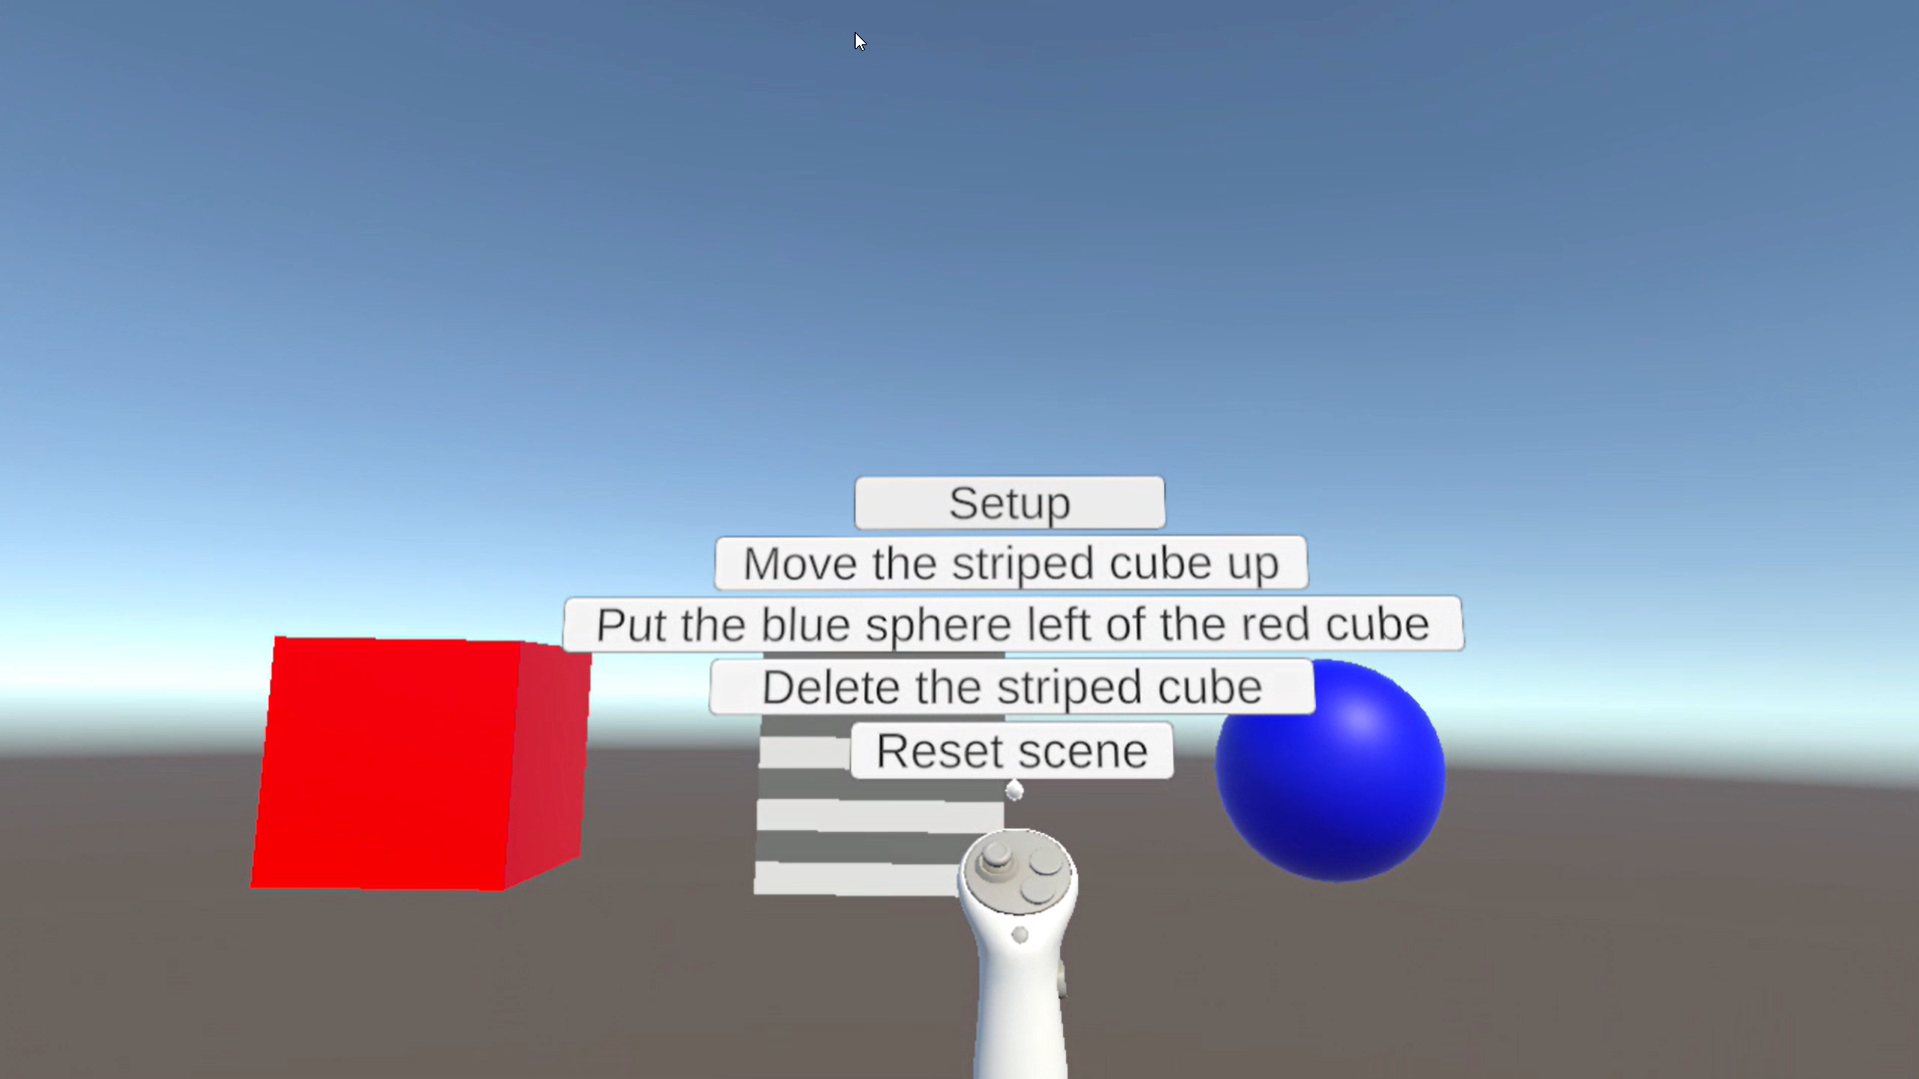
\includegraphics[width=0.7\linewidth]{figures/demo_still}
  \caption{Frühe Ausbaustufe des Demonstrators mit Bedienmenü. Links der rote Würfel, rechts die blaue Kugel; der gestreifte Würfel in der Mitte wird von der Menütafel weitgehend verdeckt, nur sein unterer Teil ist sichtbar. Das Standbild stammt aus der Aufzeichnung in Anhang~\ref{anh:video}, in der unter anderem \enquote{move the striped cube up}, \enquote{put the blue sphere left of the red cube} und \enquote{delete the striped cube} über das Menü ausgelöst werden.}
  \label{fig:demo}
\end{figure}
